\section{Factorisation LU} % (fold)
\label{sec:factorisation_lu}

\subsection{Méthode} % (fold)
\label{sub:methode}

\begin{figure}[H]
\centering
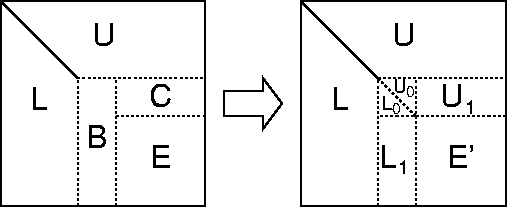
\includegraphics[width=0.8\textwidth]{lu}
\caption{Décomposition LU right-looking}
\label{fig:lu}
\end{figure}

Pour ce projet, nous utilisons la factorisation LU right-looking, illustrée par la figure \ref{fig:lu}. Nous pouvons y voir une partie de la factorisation déjà effectuée (L et U). Ensuite, nous appliquons l'algorithme expliqué (de façon simplifié) en Fig. \ref{code:lu}.

\begin{figure}[H]
\begin{lstlisting}
for (j = 0; j < MIN(m,n); j+=nb)
		dgetf2(m-j, nb, A[j, j]);
		dtrsm(Lower, nb, n-j-nb+1, A[j, j], A[j, j+nb]);
		dgemm(m-j-nb, n-j-nb, nb, A[j+nb, j], A[j, j+nb], A[j+nb, j+nb]);
\end{lstlisting}
\caption{Décomposition LU (dgetrf)}
\label{code:lu}
\end{figure}
Sur $B$, de largeur $nb$, nous effectuons une décomposition LU (dgetf2 ou dgetrf par exemple, mais ici nous avons utilisé dgetf2, étant donné que $nb$ est censé être relativement petit). Puis nous pouvons exécuter un dtrsm sur $L_0$ et $C$, essayant de résoudre l'équation \ref{eq:dtrsm}, et affectant le résultat dans $U_1$. Enfin, nous effectuons un dgemm sur $L_1$, $U_1$ et $E$, effectuant l'opération décrite dans l'équation \ref{eq:dgemm}. Puis nous itérons et réexécutons la totalité de ce procédé sur $E'$

\begin{equation}
\label{eq:dtrsm}
L_0 \times X = C
\end{equation}

\begin{equation}
\label{eq:dgemm}
E' = E - L_1 * U_1
\end{equation}

\subsection{Parallélisme} % (fold)
\label{sub:parallelisme}

Pour paralléliser les calculs sur plusieurs processeurs, une méthode est de distribuer des blocs colonnes, de largeur $nb$, et ce en serpentin. Cela signifie que les blocs colonnes seront réparties comme indiqué en Fig. \ref{fig:serpentin}.

\begin{figure}[H]
\centering
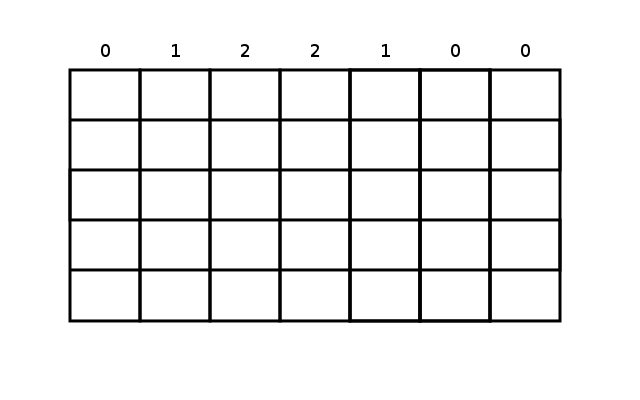
\includegraphics[width=0.8\textwidth]{serpentin}
\caption{Distribution en serpentin}
\label{fig:serpentin}
\end{figure}


